\documentclass[12pt]{article}
\usepackage[paperwidth=148mm, margin=0.5cm]{geometry} 
% Make paper smaller so everything is bigger

\usepackage[dvipsnames,rgb]{xcolor}
\usepackage{tikz}
\usetikzlibrary{positioning,shapes,arrows, fit, shapes.geometric, shadows.blur}

\usepackage{etoolbox}   
\usepackage[english]{babel}

%%%%%%%%%%%%%%%%%%%%%%%%
% Setup tcolorbox for listings
\usepackage[skins,listings]{tcolorbox}
\tcbuselibrary{minted}
\newtcblisting{demolr}[2][]{%
    text outside listing,%
    listing engine=minted,%
    minted language=tex,%
    minted options= {fontsize=\small,autogobble},%
    righthand width=0.65\textwidth,
    box align=center,
    halign=center,
    valign=center,
    center lower
}
\newtcblisting{demotb}[2][]{%\
    text above listing,
    listing engine=minted,%
    minted language=tex,%
    minted options= {fontsize=\small,autogobble, breaklines},%
    box align=center,
    halign=center,
    valign=center,
    center lower
}


%%%%%%%%%%%%%%%%%%%%%%%%%%%%%%%%%%%%%%%%%%%%%%%%%%%%%%%%%%%%%%
% Custom Slide Environment that fits pages to their content


\newenvironment{slide}[1]{%Start
	  %based on https://tex.stackexchange.com/a/299008/5834
	  \hoffset=-1in
      \voffset=-1in
      \setbox0=\vbox\bgroup%
      \begin{minipage}[t]{128mm}
      \vspace{1in}
      \section*{#1}
      \vspace{1cm}
    }{ % End
      \vspace{1in}
      \end{minipage}
      \egroup
      \pdfpageheight=\dimexpr\ht0+\dp0\relax
      \pdfpagewidth=\wd0
      \shipout\box0
}

%%%%%%%%%%%%%%%%%%%%%%%%%%%%%%%%%%%%%%%%%%%%%
% Beginning of Document Proper

\renewcommand{\familydefault}{\sfdefault}
\begin{document}

\begin{slide}{}
\begin{demotb}{}


\begin{tikzpicture}[
    every node/.style={rounded corners=7pt}]
    
    \node[draw=none, shade, 
        color=White,
        top color=Violet, bottom color=Purple,
        blur shadow={shadow blur steps=5}
    ](title) {\Huge TikZ For Diagramming};

    \node[draw, inner sep = 3mm,
        below = of title, xshift= 5cm
    ](author) {\LARGE By Lyndon White};
    
    \draw[->, very thick] (title.south)
        to[bend right=45] (author.west);
\end{tikzpicture}
\vspace{2cm}
\end{demotb}
\end{slide}

%%%%%%%%%%%%%%%%%%%%%%%%%%%%%%%%%%%%%%%%%%%%%%%%%%%%%%
\begin{slide}{What Goes into a Good Paper?}
\begin{demotb}{}
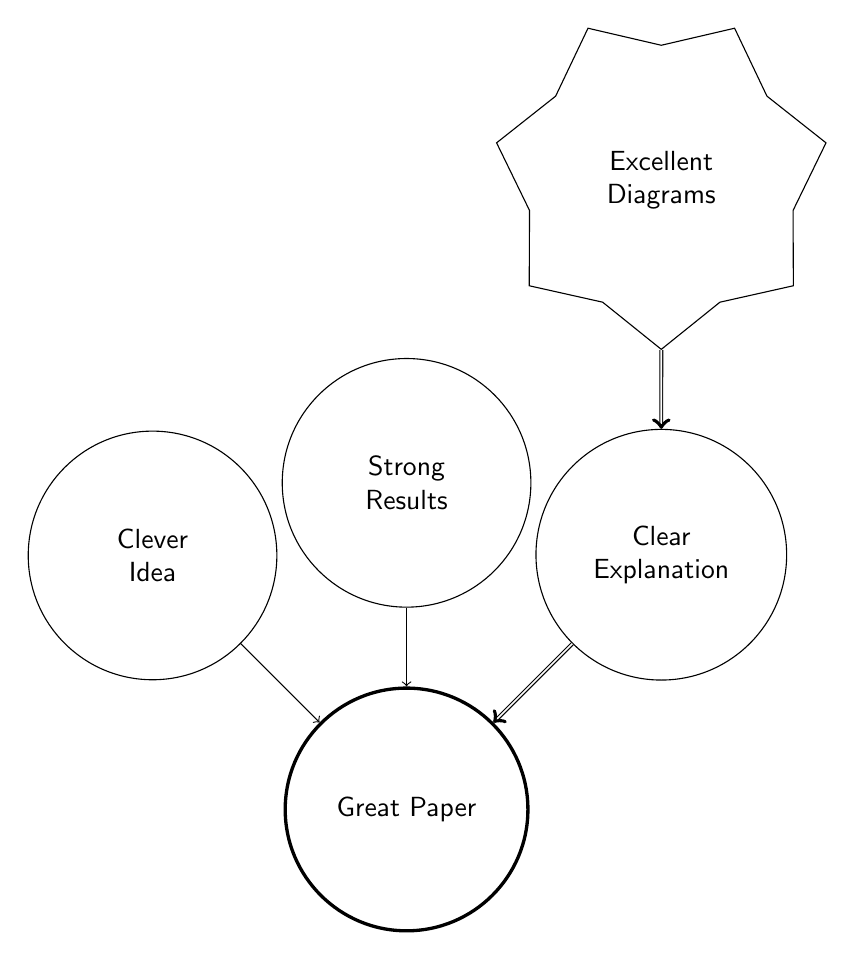
\begin{tikzpicture}[
    every node/.style={
    draw, circle, text width=2.8cm, align=center}
    ]
    
    \node[very thick](paper){Great Paper};
    \node[above left= of paper](idea) {Clever\\Idea};
    \node[above = of paper](results) {Strong\\Results};
    \node[above right= of paper](explain) {Clear\\Explanation};
    \node[above = of explain,
    star,star points=7,star point ratio=0.8
    ](diagram){Excellent\\Diagrams};

    \draw[->, double] (diagram) -> (explain);
    \draw[->, double] (explain)->(paper);
    \draw[->] (results)->(paper);
    \draw[->] (idea)->(paper);
\end{tikzpicture}
\vspace{1cm}
\end{demotb}
\end{slide}

%%%%%%%%%%%%%%%%%%%%%%%%%%%%%%%%%%%%%%%%%%

\begin{slide}{PGF/TikZ Ecosystem}
\begin{demotb}{}
    \newcommand{\sublist}[2]{
        \foreach \name[count=\ii from 1] in {#2}
        {
            \node[below=\ii of #1.east] (\name) {\texttt{\name}};
            \draw (#1.south) to[tl] (\name);
        }
    }
    \resizebox{\textwidth}{!}{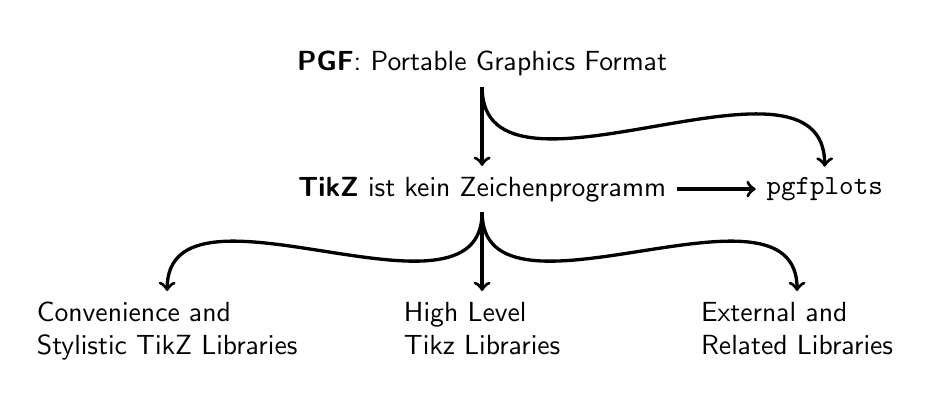
\begin{tikzpicture}[
        ->, very thick,
        tt/.style={out=-90,in=90},
        tl/.style={out=-90,in=180},
        every node/.style={align=left}
    ]
    \node(pgf) {\textbf{PGF}: Portable Graphics Format};
    \node[below=of pgf](tikz) {\textbf{TikZ} ist kein Zeichenprogramm};
    \node(pgfplots)[right=of tikz]{\texttt{pgfplots}};
    
    
    \draw (pgf) to[tt] (tikz);
    \draw (pgf) to[tt] (pgfplots);
    \draw (tikz) to (pgfplots);
    
    
    
    \node[below=of tikz, xshift=-4.cm] (stylelibs) {Convenience and\\ Stylistic TikZ Libraries};
    \draw (tikz) to[tt] (stylelibs);
    \sublist{stylelibs}{fit, shapes, arrows, shadows, matrix, positioning, decoration}
    
    \node[below=of tikz, xshift=0cm] (highlibs) {High Level\\ Tikz Libraries};
    \draw (tikz) to[tt] (highlibs);
    \sublist{highlibs}{chains,graphs,trees,automata, circuit, mindmap}
    
        
    \node[below=of tikz, xshift=4.cm] (highlibs) {External and \\ Related Libraries};
    \draw (tikz) to[tt] (highlibs);
    \sublist{highlibs}{tikz-cd, Beamer*, pgfgantt, tikzposter}
    
    \end{tikzpicture}}
    \vspace{1cm}
    \end{demotb}

\end{slide}


%%%%%%%%%%%%%%%%%%%%%%%%%%%%%%%%%%%%%%%%%%%

\begin{slide}{What is so great about TikZ?}
\begin{demotb}{}
    \def\ppos{-3.5}
    \def\cpos{3.5}
    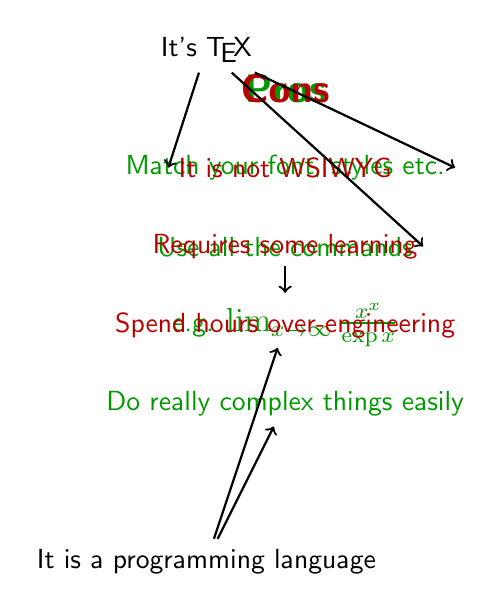
\begin{tikzpicture}[->, thick,
        pro/.style={color=OliveGreen},
        con/.style={color=BrickRed}    
    ]
    \node[pro] at (\ppos, 0) {\Large\textbf{Pros}};
    \node[pro](p1) at (\ppos, -1) {Match your font, styles etc.};
    \node[pro](p2) at (\ppos, -2) {Use all the commands};
    \node[pro](p3) at (\ppos, -3) {
        e.g. \large $\lim_{x\to \infty} \frac{x^x}{\exp x}$
    };
    \node[pro](p4) at (\ppos, -4) {Do really complex things easily};
   
    \draw[->] (p2) -- (p3);
    
    \node(t1) at (0, 0.5) {It's \TeX};
    \node(t2) at (0, -6) {It is a programming language};
    
    \node[con] at (\cpos,0) {\Large \textbf{Cons}}; 
    \node[con](c1) at (\cpos,-1) {It is not WSIWYG};
    \node[con](c2) at (\cpos, -2) {Requires some learning};
    \node[con](c3) at (\cpos, -3) {Spend hours over-engineering};
    
    
    \draw (t1) -- (c1.west);
    \draw (t1) -- (p1.east);
    \draw (t1) -- (p2.east);
    
    \draw (t2) -- (c3); 
    \draw (t2) -- (p4);
    
    \end{tikzpicture}
    \vspace{1cm}
\end{demotb}
\end{slide}




%%%%%%%%%%%%%%%%%%%%%%%%%%%%%%%%%%%%%%%%%%%

\begin{slide}{Basics: Loading the package}
    \begin{minted}{tex}
        \documentclass{article}
        \usepackage{tikz}
        \usetikzlibrary{positioning}
        % Always use positioning library
        %...
        %...
        \begin{document}
        %...
        %...
        %...
     
        \begin{figure}
        %Maybe a \resizebox here or similar
        \begin{tikzpicture}
        %...
        % WRITE YOUR DIAGRAM TikZ CODE HERE
        % THIS IS WHERE THE MAGIC GOES
        %...
        \end{tikzpicture}
        \caption{Figures should have captions}
        \end{figure}
        %...
        %...
        %...
        \end{document}
    \end{minted}
\end{slide}

% %%%%%%%%%%%%%%%%%%%%%%%%%%

\begin{slide}{Basics: A node}
    \begin{demolr}{}
    
\begin{tikzpicture}
        \node[](name) at (0,0) {content};
    \end{tikzpicture}
    \end{demolr}
    \vspace{1cm}

    \begin{demolr}{}
    
\begin{tikzpicture}
        \node{I am a node};
    \end{tikzpicture}
    \end{demolr}
    \vspace{1cm}
    \begin{demolr}{}
    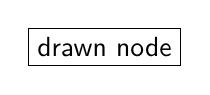
\begin{tikzpicture}
        \node[draw]{drawn node};
    \end{tikzpicture}
    \end{demolr}
    \vspace{1cm}
    \begin{demolr}{}
    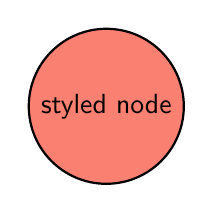
\begin{tikzpicture}
        \node[draw, circle, thick,
        fill=Salmon,
        ]{styled node};
    \end{tikzpicture}
    \end{demolr}
    \vspace{1cm}
    \begin{demolr}{}
    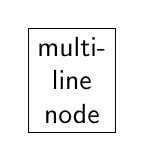
\begin{tikzpicture}
        \node[draw,
            align=center %got to set align
        ]{multi-\\line\\node};
    \end{tikzpicture}
    \end{demolr}
\end{slide}

%%%%%%%%%%%%%%%%%%%%%%%%%%%%%%%%%%%%%%%%%%%

\begin{slide}{Defining styles}

\subsection*{Locally}
\begin{demolr}{}
    
\begin{tikzpicture}[
        input/.style={draw, thick,Purple}
    ]
    \node[input]{I am a node};
    \end{tikzpicture}
\end{demolr}

\subsection*{Globally}
\begin{demolr}{}
    \tikzset{input/.style={draw, thick, Orange}}
    
    \begin{tikzpicture}
        \node[input]{pict 1};
    \end{tikzpicture}
    
    \begin{tikzpicture}
        \node[input]{pict 2};
    \end{tikzpicture}
    
    \begin{tikzpicture}
        \node[input, OliveGreen]{pict 3};
    \end{tikzpicture}
\end{demolr}

\subsection*{Via Rule}
\begin{demolr}{}
    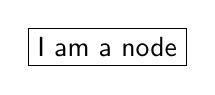
\begin{tikzpicture}[
        every node/.style={draw}
    ]
    \node{I am a node};
    \end{tikzpicture}
\end{demolr}

\end{slide}
%%%%%%%%%%%%%%%%%%%%%%%%%%%%%%%%%%%%%%%%%%%%%

\begin{slide}{Positioning}
    \subsection*{Absolute}
    \begin{demotb}{}
    \begin{tikzpicture}[every node/.style = {draw}]
        \node at (-1,1) {first};
        \node at (1,4) {second};
        \node at (7,2) {third};
    \end{tikzpicture}
    \end{demotb}
    \vspace{1cm}
    \subsection*{Relative}
    \begin{demotb}{}
    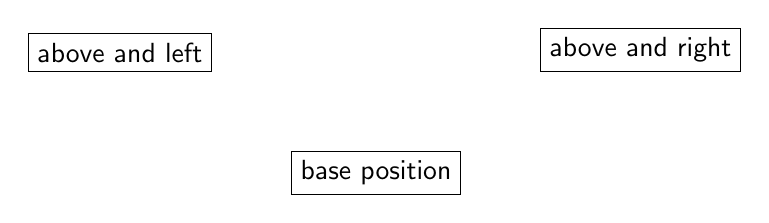
\begin{tikzpicture}[every node/.style = {draw}]
        \node(first) {base position};
        \node[above left = of first] {above and left};
        \node[above right = of first]{above and right};
    \end{tikzpicture}
    \end{demotb}

    \vspace{2cm}
    \begin{demotb}{}
    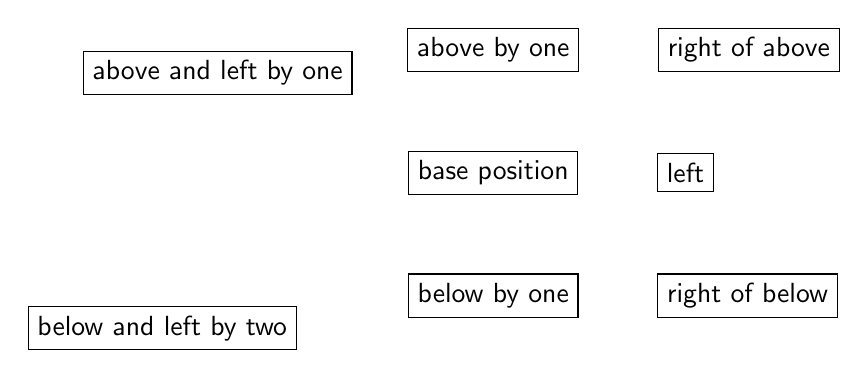
\begin{tikzpicture}[every node/.style = {draw}]
        \node(first) {base position};         
        \node(ab)[above = 1 of first]{above by one};
        \node[right = of ab]{right of above};
        \node[right = of first]{left};
        \node(bl)[below = 1 of first]{below by one};
        \node[right = of bl]{right of below};
        
        \node[above left = 1 of first] {above and left by one};
        \node[below left = 2 of first] {below and left by two};
        
    \end{tikzpicture}
    \end{demotb}
    
    \vspace{1cm}
    \subsection*{Nudging}
    \begin{demotb}{}
    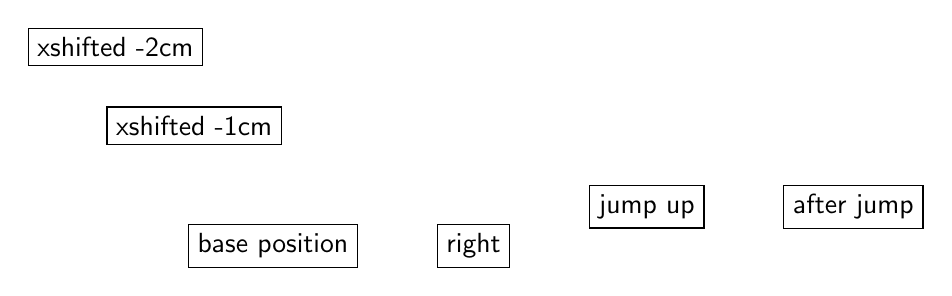
\begin{tikzpicture}[every node/.style = {draw}]
        \node(first) {base position};
        \node[above = 2 of first, xshift=-2cm] {xshifted -2cm};
        \node[above = 1 of first, xshift=-1cm] {xshifted -1cm};
        
        \node(second) [right = of first] {right};
        \node(third) [right = of second, yshift=5mm] {jump up};
        \node(fourth) [right = of third] {after jump};
    \end{tikzpicture}
    \end{demotb}
    
\end{slide}


%%%%%%%%%%%%%%%%%%%%%%%%%%%%%%%%%%%%%%%%%%%%%%%%%%%%%%

\begin{slide}{Drawing connectors:\\ Attaching things to things}

\begin{demolr}{}
    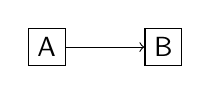
\begin{tikzpicture}
        \node[draw](a){A};
        \node[draw, right=of a](b){B};
        \draw[->] (a) to (b);
    \end{tikzpicture}
\end{demolr}

\begin{demolr}{}
    \begin{tikzpicture}
        \node[draw](a){A};
        \node[draw, below right=2 of a](b){B};
        \draw[->] (a) -| (b);
    \end{tikzpicture}
\end{demolr}

\begin{demolr}{}
    \begin{tikzpicture}
        \node[draw](a){A};
        \node[draw, below right=2 of a](b){B};
        \draw[->] (a) to[bend right] (b);
    \end{tikzpicture}
\end{demolr}

\end{slide}

% %%%%%%%%%%%%%%%%%%%%%%%%%%%%%%%%%%%%%%%%%%%%%%%%

\begin{slide}{Put a label on that connector}
\begin{demolr}{}
    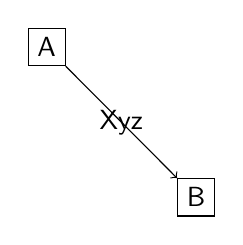
\begin{tikzpicture}
        \node[draw](a){A};
        \node[draw, below right=2 of a](b){B};
        \draw[->] (a) to node {Xyz} (b);
    \end{tikzpicture}
\end{demolr}

\begin{demolr}{}
    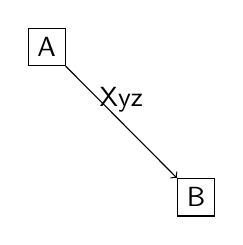
\begin{tikzpicture}
        \node[draw](a){A};
        \node[draw, below right=2 of a](b){B};
        \draw[->] (a) to node[above] {Xyz} (b);
    \end{tikzpicture}
\end{demolr}

\begin{demolr}{}
    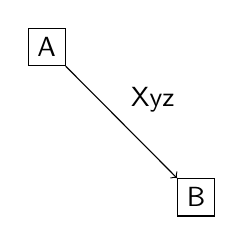
\begin{tikzpicture}
        \node[draw](a){A};
        \node[draw, below right=2 of a](b){B};
        \draw[->] (a) to node[auto] {Xyz} (b);
    \end{tikzpicture}
\end{demolr}

\vspace{2cm}

\subsection*{Styling the edge node, to grey-out lines behind it}
\subsubsection*{Via  named style}
\begin{demolr}{}
    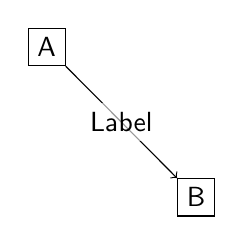
\begin{tikzpicture}[
        labe/.style={
            fill=White,
            fill opacity=0.6,
            text opacity=1}
    ]
        \node[draw](a){A};
        \node[draw, below right=2 of a](b){B};
        \draw[->] (a) to node[labe] {Label} (b);
    \end{tikzpicture}
\end{demolr}

\subsubsection*{Via rule}
\begin{demolr}{}
    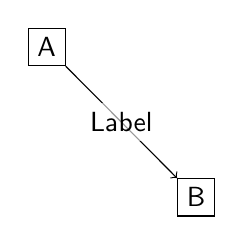
\begin{tikzpicture}[
        every to/.append style = {
            every node/.style={
                fill=White,
                fill opacity=0.6,
                text opacity=1
            }
        }
    ]
        \node[draw](a){A};
        \node[draw, below right=2 of a](b){B};
        \draw[->] (a) to node {Label} (b);
    \end{tikzpicture}
\end{demolr}

\end{slide}

%%%%%%%%%%%%%%%%%%%%%%%%%%

\begin{slide}{Coordinates and Anchors}
\begin{demolr}{}
    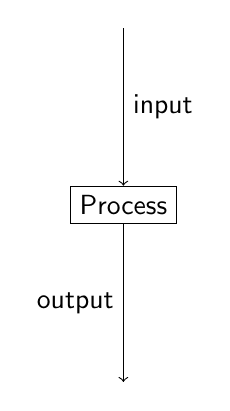
\begin{tikzpicture}
        \coordinate(a) at (0,0);
        \node[draw, below = 2 of a](b){Process};
        \coordinate[below = 2 of b](c);
    
        \draw[->](a) to node[right] {input} (b);
        \draw[->](b) to node[left] {output} (c);
    \end{tikzpicture}
\end{demolr}

\begin{demolr}{}
    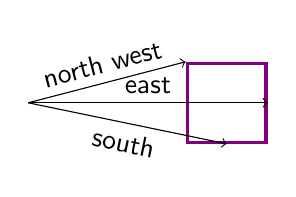
\begin{tikzpicture}
        \coordinate(a) at (0,0);
        \node[draw, right = 2 of a, 
            Purple, very thick,
            minimum size=1cm](b){};
    
        \draw[->] (a) 
            to node[above] {east}
            (b.east);
        \draw[->] (a) 
            to node[sloped, above] {north west}
            (b.north west);
        \draw[->] (a) 
            to node[sloped, below] {south}
            (b.south);
    \end{tikzpicture}
\end{demolr}

\begin{demolr}{}
    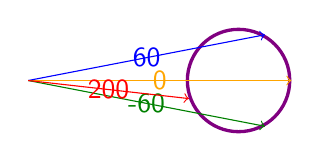
\begin{tikzpicture}[->]
        \coordinate(a) at (0,0);
        \node[draw, right = 2 of a, 
            Purple, very thick, circle,
            minimum size=1.3cm](b){};
    
        \draw[Orange] (a) to node {0} (b.0);
        \draw[Blue] (a) to node {60} (b.60);
        \draw[Green] (a) to node {-60} (b.-60);
    
        \draw[Red] (a) to node {200} (b.200);
    \end{tikzpicture}
\end{demolr}
\end{slide}

%%%%%%%%%%%%%%%%%%%%%%%%%%%%%%%%%%%%%%%%%%%%%

\begin{slide}{Loops 1: Basics}

\begin{demotb}{}
    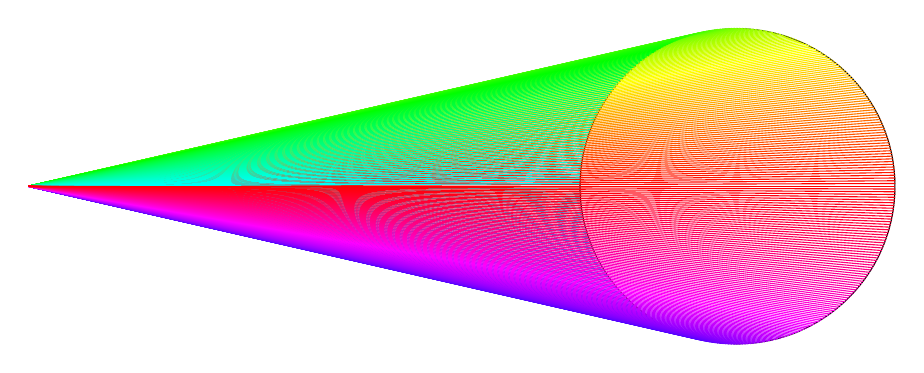
\begin{tikzpicture}
    \coordinate(a) at (0,0);
    \node[draw,circle, right = 7cm of a, minimum size=4cm](b){};
    
    \foreach \ii in {1,...,360}{
        \definecolor{linecolor}{Hsb}{\ii,1,1};    
        %^ requires \usepackage[rgb]{xcolor}
        \draw[color=linecolor] (a) to (b.\ii);
    }
    \end{tikzpicture}
\end{demotb}

\vspace{2cm}

\begin{demotb}{}
    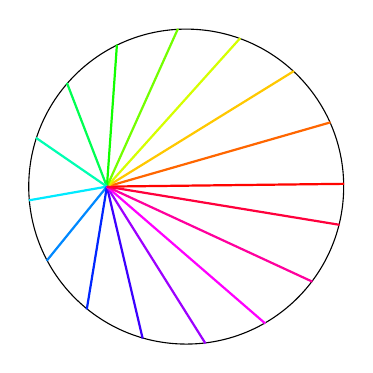
\begin{tikzpicture}
    \coordinate(a) at (0,0);
    \node[draw,circle, right = -1cm of a, minimum size=4cm](b){};
    
    \foreach \ii in {1,24,...,360}{
        \definecolor{linecolor}{Hsb}{\ii,1,1};    
        %^ requires \usepackage[rgb]{xcolor}
        \draw[color=linecolor, thick] (a) to (b.\ii);
    }
    \end{tikzpicture}
\end{demotb}

\end{slide}

%%%%%%%%%%%%%%%

\begin{slide}{Loops 2: Making Diagrams with Connections}
\subsection*{Absolute positioning}
\begin{demotb}{}
    
\begin{tikzpicture}
    \foreach \curr in {0, ..., 4} {
        \node (L\curr) at (2*\curr, 0) {Layer \curr};
    }
    \end{tikzpicture}
\end{demotb}

\subsection*{Iterating Tuples via /}
\begin{demotb}{}
    
\begin{tikzpicture}[
        title/.style={text width=1.8cm, align=center, font=\small}
    ]
        \node[title] (L0) {One-Hot\\Input};
        \foreach \curr/\prev/\content in {
                1/0/{Input\\ Embeddings}, 
                2/1/{Abstract\\Representation},
                3/2/{Output\\ Embeddings},
                4/3/{Softmax Output}
                } {
            \node[title, right= 0.6 of L\prev] (L\curr) { \content};
            \draw[->] (L\prev) to (L\curr);
        }
    \end{tikzpicture}
\end{demotb}

\subsection*{Using 0 based-count to get previous, from 1 based}
\begin{demotb}{}
    
\begin{tikzpicture}
        \node (L0) {Layer 0};
    \foreach \curr [count=\prev from 0] in {1, ..., 4} {
        \node[right=of L\prev] (L\curr) {Layer \curr};
        \draw[->] (L\prev) to (L\curr);
    }
    \end{tikzpicture}
\end{demotb}

\subsection*{Nested Loops}
\begin{demotb}{}
    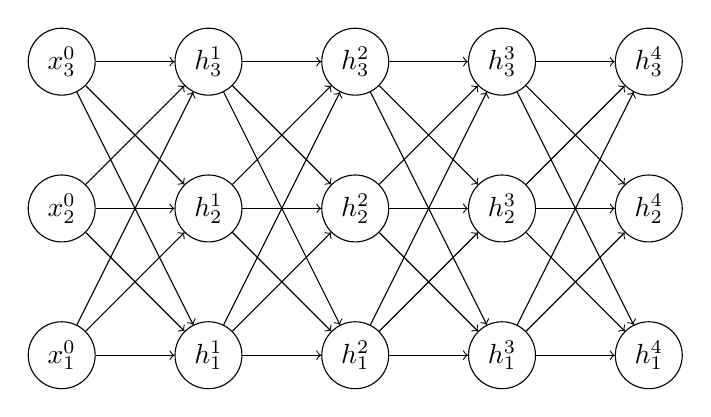
\begin{tikzpicture}[every node/.style={draw, circle}]
        % First (left-side) layer
        \coordinate (L_0_0) at (0,0);
        \foreach \ii [count=\previi from 0] in {1,...,3}{
            \node[above=of L_0_\previi] (L_0_\ii) {$x^0_\ii$};
        }
        % other layers
        \foreach \curr [count=\prev from 0] in {1, ..., 4} {
            \foreach \ii [count=\previi from 0] in {1,...,3}{
                % each node on curr layer
                \node[right=of L_\prev_\ii] (L_\curr_\ii) {$h^\curr_\ii$};
            
                \foreach \jj in {1,...,3}{
                    % each node on prev layer
                    \draw[->] (L_\prev_\jj) to (L_\curr_\ii);
                }
            }
        }
    \end{tikzpicture}
\end{demotb}

\end{slide}
%%%%%%%%%%%%%%%%%%%%%%%%%%%%%%%%%%%%%%%%%%%%%%%%%%

\begin{slide}{Pathway to madness: flexible layer sizes\\ by adding in control flow and math}
This uses the \texttt{etoolbox} package.
Similar can be done with other math and control packages.
I like \texttt{etoolbox} better than e.g. the \texttt{pgfmath} stuff that comes with TikZ.

\begin{demotb}{}
    
    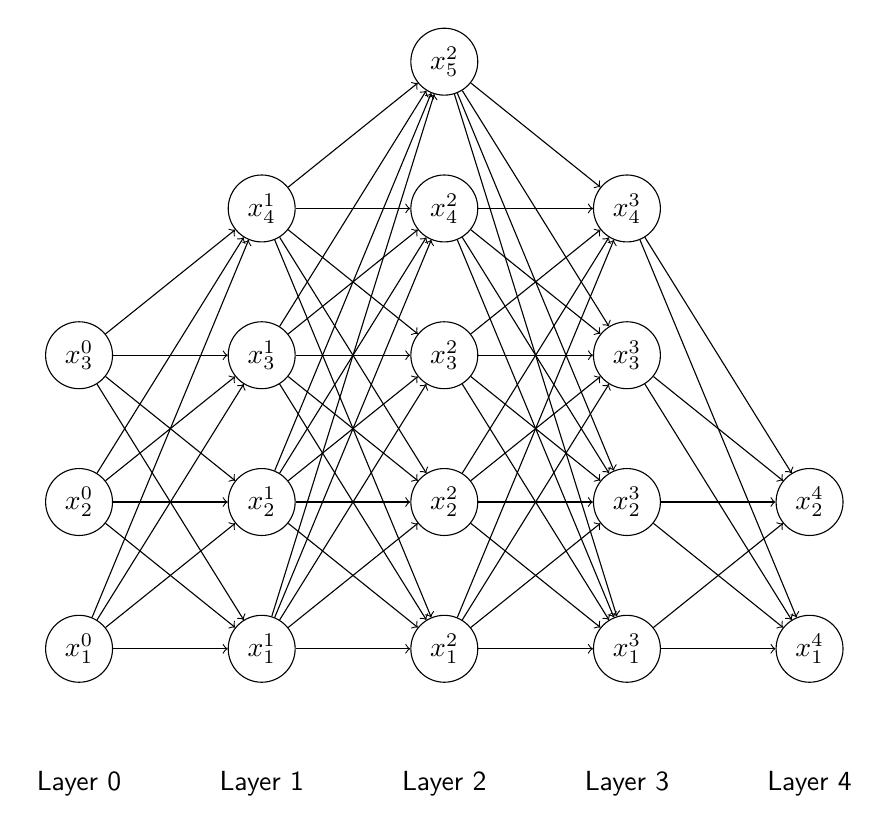
\begin{tikzpicture}   
        \foreach \currlayer/\numitems in {0/3,1/4,2/5,3/4,4/2}
        {
            % ==Draw labels on the bottom==
            \ifnumcomp{\currlayer}{>}{0}
            {% Layers after the first
                \numgdef{\prevlayer}{\currlayer-1}    
                \node[right=of L_\prevlayer_0] (L_\currlayer_0) {Layer \currlayer};
            }
            {% Layer 0 only
                \node (L_0_0) at (0,0) {Layer 0};
            }
        	
            % ==Draw the layers nodes==
            \foreach \ii in {1,...,\numitems}{
                \numdef{\previi}{\ii-1}    
                    \node[draw,circle, above=of L_\currlayer_\previi] (L_\currlayer_\ii) {$x^\currlayer_\ii$};
            
            	% ==Draw in connections==
                \ifnumcomp{\currlayer}{>}{0}
                {% Layers after the first
                    \foreach \jj in {1,...,\prevnumitems} {
                        \draw[->] (L_\prevlayer_\jj) to (L_\currlayer_\ii);
                    }
                }
                {}%Layer 0 only, nothing extra
            }
            \numgdef{\prevnumitems}{\numitems}
         }
    \end{tikzpicture}
\end{demotb}
\end{slide}

%%%%%%%%%%%%%%%%%%%%%%%%%%%%%%%%%%%%%%%%%%%

\begin{slide}{Bonus Figure: Relationship Graph}
    \begin{demotb}{}
        \tikzset{
        every picture/.style={/utils/exec={\sffamily}},
        every matrix/.style={ampersand replacement=\&, rounded corners=10pt},
        every node/.style = {font=\scriptsize, inner sep = 3},
        >=latex
        }
        \resizebox{\textwidth}{!}{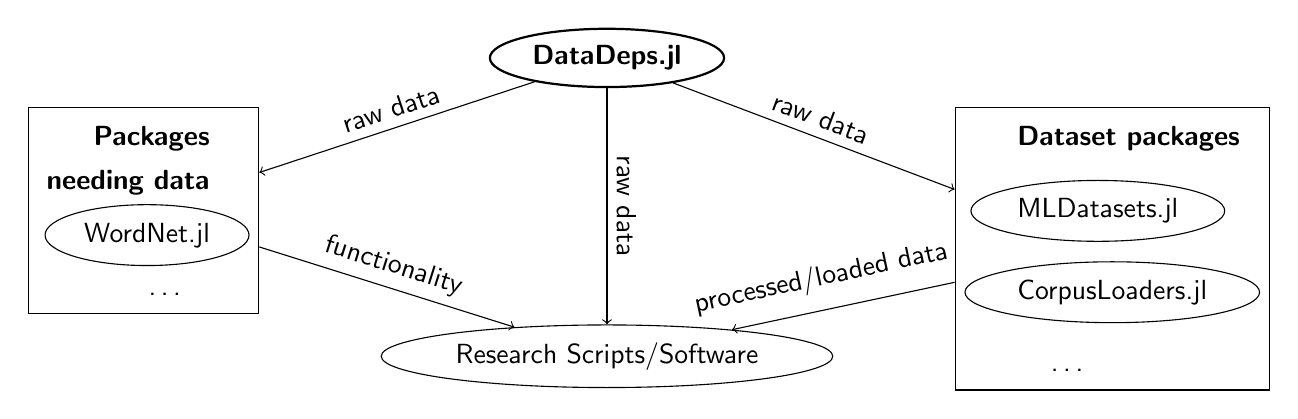
\begin{tikzpicture}[]
        \node[ellipse, thick, draw, inner sep = 3] (datadeps) {\textbf{DataDeps.jl}};
        \node[matrix, xshift=3cm, below right = 0.5 of datadeps, draw, column sep=15, row sep=7] (datasetpackages) {
            \node{\textbf{Dataset packages}}; \\
            \node[draw,ellipse]{MLDatasets.jl};\\
            \node[draw,ellipse]{CorpusLoaders.jl}; \\
            \node{\phantom{M} \ldots \phantom{M}};\\
        };
        \node[matrix, xshift=-3cm, below left = 0.5 of datadeps, draw, column sep=15] (packages) {
            \node{\textbf{Packages}}; \\
            \node{\textbf{needing data}}; \\
            \node[draw,ellipse]{WordNet.jl}; \\
            \node{\phantom{M} \ldots \phantom{M}};\\
        };
        \node[ellipse, draw, inner sep = 3, below = 3 of datadeps] (researchcode) {Research Scripts/Software};
        
        \path[->,draw] (datadeps) edge node[sloped,above]{raw data} (packages);
        \path[->,draw] (packages) edge node[sloped,above]{functionality} (researchcode);
        
        \path[->,draw] (datadeps) edge[above] node[sloped,above]{raw data} (datasetpackages);
        \path[->,draw] (datasetpackages) edge[above] node[sloped,above, xshift=-0.2cm, yshift=0.1cm]{processed/loaded data} (researchcode);
        
        \path[->,draw] (datadeps) edge node[sloped,above]{raw data} (researchcode);    
        \end{tikzpicture}}
    \end{demotb}
    
\end{slide}

%%%%%%%%%%%%%%%%%%%%%%%%%%%%%%%%%%%%%%%%%%%%%%

\begin{slide}{Bonus Figure: Block Diagram}
    \begin{demotb}{}
    \newcommand{\datadep}[1]{\texttt{datadep"{}#1"{}}}
    \tikzset{
        every picture/.style={/utils/exec={\sffamily}},
        every matrix/.style={ampersand replacement=\&, rounded corners=10pt},
        every node/.style = {font=\scriptsize, inner sep = 3},
        >=latex
    }
    \resizebox{\textwidth}{!}{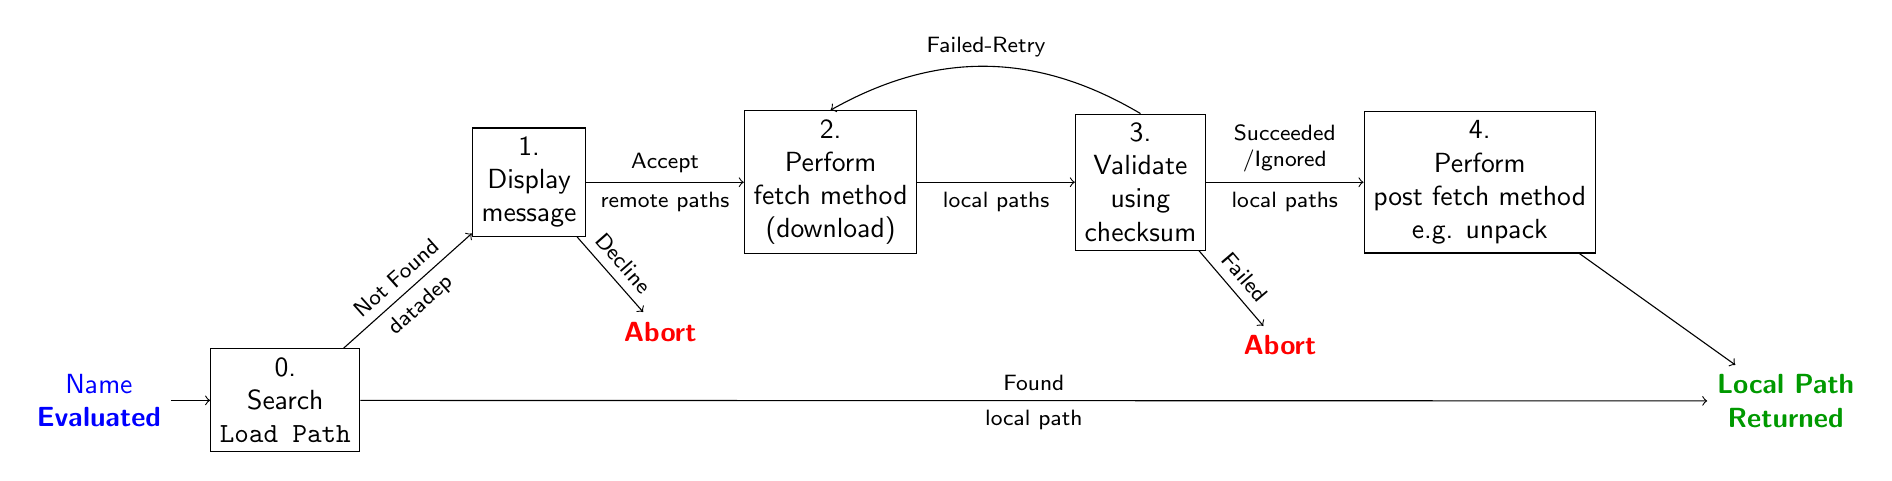
\begin{tikzpicture}[
        ->,
        every text node part/.style={align=center},
        auto,node distance=2,
        every edge/.append style={every node/.style={font=\footnotesize}}]


        \node[blue](start) {\datadep{Name}\\ \textbf{Evaluated}}; 

        \node[draw, rectangle, right= 0.5 of start] (search) {0.\\Search\\ \texttt{Load Path}};
        \node[draw, rectangle, above right= of search] (msg) {1.\\Display\\ message};
        \node[draw, rectangle, right= of msg] (fetch) {2.\\Perform\\ fetch method\\ (download)};
        \node[draw, rectangle, right= of fetch] (checksum) {3.\\Validate\\ using\\ checksum};
        \node[draw, rectangle, right= of checksum] (postfetch) {4.\\Perform \\post fetch method\\ e.g. unpack};
        \node[green!60!black, below right=of postfetch](end) {\textbf{Local Path}\\ \textbf{Returned}};

        \path (start) edge (search);
        \path (search) edge node[sloped,below]{datadep} node[sloped,above]{Not Found} (msg);
        \path (msg) edge[below] node{remote paths} node[above]{Accept} (fetch);
        \path (fetch) edge[below] node{local paths} (checksum);
        \path (checksum) edge node[below]{local paths} node[above]{Succeeded\\/Ignored} (postfetch);
        \path (postfetch) edge (end);
        \path (search) edge node[above]{Found} node[below]{local path} (end);


        \path (checksum.north) edge[bend right] node[above] {Failed-Retry} (fetch.north);

        \node[red, below right = 0.5 of msg, yshift=-0.6cm] (err1) {\textbf{Abort}};
        \path (msg) edge node[above, sloped]{Decline} (err1);

        \node[red, below right = 0.5 of checksum, yshift=-0.6cm] (err2) {\textbf{Abort}};
        \path (checksum) edge node[above, sloped]{Failed} (err2);
        \end{tikzpicture}}
    \end{demotb}
\end{slide}

%%%%%%%%%%%%%%%%%%%%


\begin{slide}{Bonus Figure:\\ Neural Network High Level Structure}
    
    \begin{demotb}{}

    \newcommand{\picwidth}{60pt}
    \begin{tikzpicture}[%
        node distance=1cm and 1.5cm,
        every text node part/.style= {align=center},
        word/.style= {blue, font=\itshape,},
        layer/.style= {rectangle, black,draw},
    ]

        \node (hiddenoutput)[layer] at (0,0) {ReLU};
        \node (GRU1)[layer, below = of hiddenoutput]{GRU};

        \foreach[count=\i from 1] \j in {2,...,4}
        {
            \node (GRU\j)[layer, left = of GRU\i]{GRU};
            \draw[->] (GRU\j) to (GRU\i);
        }

        \foreach[count=\i from 1] \word in {green, ish, blue, light}
        {
            \node (emb\i)[layer, below = of GRU\i]    {Embedding};
            \node (word\i)[word, below = of emb\i]{\word};
            \draw[->] (word\i) to    (emb\i);
            \draw[->] (emb\i) to (GRU\i);
            \node[draw,dotted,fit= (emb\i) (word\i) (GRU\i)] {};
        }


        \draw[->] (GRU1) to (hiddenoutput);

        \node(outHue)[layer, above left = of hiddenoutput] {Softmax};
        \node(outSaturation)[layer, above = of hiddenoutput] {Softmax};
        \node(outValue)[layer, above right = of hiddenoutput] {Softmax};

        \foreach \p in {Hue, Saturation, Value} 
        {
            \draw[->] (hiddenoutput) to (out\p);

            \node(plot\p)[above = of out\p, text width=\picwidth]{
                \includegraphics[width=\picwidth]{netdia/\p}
                \\
                \p
                };
            \draw[->] (out\p) to (plot\p);
        }
    \end{tikzpicture}
    \end{demotb}
    
    
\end{slide}


\end{document}